%% LyX 2.3.4.2 created this file.  For more info, see http://www.lyx.org/.
%% Do not edit unless you really know what you are doing.
\documentclass[english,dvipsnames,aspectratio=169]{beamer}
\usepackage{mathptmx}
\usepackage{eulervm}
\usepackage[T1]{fontenc}
\usepackage[latin9]{inputenc}
\usepackage{babel}
\usepackage{amstext}
\usepackage{amssymb}
\usepackage{graphicx}
\usepackage{ifthen}
\usepackage{xcolor}
\usepackage{xspace}
\usepackage{tikz}
\usetikzlibrary{tikzmark}
\usetikzlibrary{calc}
\usepackage{pgfplots}
%\pgfplotsset{compat=1.17}
\usepackage{booktabs}
\usepackage{xpatch}

\xpatchcmd{\itemize}
  {\def\makelabel}
  {\ifnum\@itemdepth=1\relax
     \setlength\itemsep{2ex}% separation for first level
   \else
     \ifnum\@itemdepth=2\relax
       \setlength\itemsep{1ex}% separation for second level
     \else
       \ifnum\@itemdepth=3\relax
         \setlength\itemsep{0.5ex}% separation for third level
   \fi\fi\fi\def\makelabel
  }
 {}
 {}

\ifx\hypersetup\undefined
  \AtBeginDocument{%
    \hypersetup{unicode=true,pdfusetitle,
 bookmarks=true,bookmarksnumbered=false,bookmarksopen=false,
 breaklinks=false,pdfborder={0 0 0},pdfborderstyle={},backref=false,colorlinks=true,
 allcolors=NYUPurple,urlcolor=LightPurple}
  }
\else
  \hypersetup{unicode=true,pdfusetitle,
 bookmarks=true,bookmarksnumbered=false,bookmarksopen=false,
 breaklinks=false,pdfborder={0 0 0},pdfborderstyle={},backref=false,colorlinks=true,
 allcolors=NYUPurple,urlcolor=LightPurple}
\fi

\makeatletter

%%%%%%%%%%%%%%%%%%%%%%%%%%%%%% LyX specific LaTeX commands.
%% Because html converters don't know tabularnewline
\providecommand{\tabularnewline}{\\}

%%%%%%%%%%%%%%%%%%%%%%%%%%%%%% Textclass specific LaTeX commands.
% this default might be overridden by plain title style
\newcommand\makebeamertitle{\frame{\maketitle}}%
% (ERT) argument for the TOC
\AtBeginDocument{%
  \let\origtableofcontents=\tableofcontents
  \def\tableofcontents{\@ifnextchar[{\origtableofcontents}{\gobbletableofcontents}}
  \def\gobbletableofcontents#1{\origtableofcontents}
}

%%%%%%%%%%%%%%%%%%%%%%%%%%%%%% User specified LaTeX commands.
\usetheme{CambridgeUS} 
\beamertemplatenavigationsymbolsempty


% Set Color ==============================
\definecolor{NYUPurple}{RGB}{87,6,140}
\definecolor{LightPurple}{RGB}{165,11,255}


\setbeamercolor{title}{fg=NYUPurple}
\setbeamercolor{frametitle}{fg=NYUPurple}

\setbeamercolor{background canvas}{fg=NYUPurple, bg=white}
\setbeamercolor{background}{fg=black, bg=NYUPurple}

\setbeamercolor{palette primary}{fg=black, bg=gray!30!white}
\setbeamercolor{palette secondary}{fg=black, bg=gray!20!white}
\setbeamercolor{palette tertiary}{fg=gray!20!white, bg=NYUPurple}

\setbeamertemplate{headline}{}
\setbeamerfont{itemize/enumerate body}{}
\setbeamerfont{itemize/enumerate subbody}{size=\normalsize}

\setbeamercolor{parttitle}{fg=NYUPurple}
\setbeamercolor{sectiontitle}{fg=NYUPurple}
\setbeamercolor{sectionname}{fg=NYUPurple}
\setbeamercolor{section page}{fg=NYUPurple}
%\setbeamercolor{description item}{fg=NYUPurple}
%\setbeamercolor{block title}{fg=NYUPurple}

\setbeamertemplate{blocks}[rounded][shadow=false]
\setbeamercolor{block body}{bg=normal text.bg!90!NYUPurple}
\setbeamercolor{block title}{bg=NYUPurple!30, fg=NYUPurple}



\AtBeginSection[]{
  \begin{frame}
  \vfill
  \centering
\setbeamercolor{section title}{fg=NYUPurple}
 \begin{beamercolorbox}[sep=8pt,center,shadow=true,rounded=true]{title}
    \usebeamerfont{title}\usebeamercolor[fg]{title}\insertsectionhead\par%
  \end{beamercolorbox}
  \vfill
  \end{frame}
}

\makeatother

\setlength{\parskip}{\medskipamount} 

\input ../macros

\begin{document}
\input ../rosenberg-macros

\title[DS-GA 1003]{What is Machine Learning}
\author{He He}
\date{\today}
\institute{CDS, NYU}

\makebeamertitle
\mode<article>{Just in article version}

\begin{frame}{Contents}
\tableofcontents{}
\end{frame}

\begin{frame}{Machine Learning Problems}

\textbf{Common theme} is to solve a prediction problem:
\begin{itemize}
\item given an \textbf{input} $x$,
\item \textbf{predict} an \textbf{output $y$.} 
\end{itemize}

We'll start with a few canonical examples...
\end{frame}
%

\begin{frame}{Example: Spam Detection}

\begin{itemize}
\item \textbf{Input:} Incoming email
\end{itemize}
\begin{center}
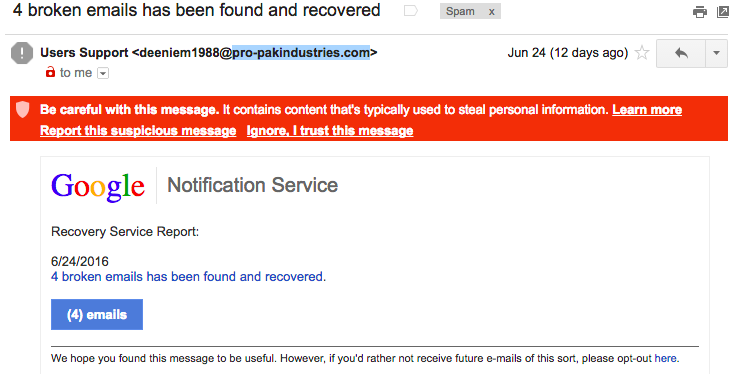
\includegraphics[width=0.6\textwidth]{figures/spam-email}
\end{center}

\begin{itemize}
\item \textbf{Output: }``SPAM'' or ``NOT SPAM''
\item A \textbf{binary classification} problem, because only 2
possible outputs.
\end{itemize}
\end{frame}

\begin{frame}{Example: Medical Diagnosis}
\begin{itemize}
\item \textbf{Input}: Symptoms (fever, cough, fast breathing, shaking, nausea, ...)

\item \textbf{Output:} Diagnosis (pneumonia, flu, common cold, bronchitis, ...)

\item A \textbf{multiclass classification} problem: choosing one of several \emph{discrete} outputs.
\end{itemize}

\medskip
How to express uncertainty?
\begin{itemize}
\item \textbf{Probabilistic classification} or \textbf{soft classification}:
\begin{eqnarray*}
\text{\ensuremath{\pr}(pneumonia)} & = & 0.7\\
\text{\ensuremath{\pr}(flu)} & = & 0.2\\
\vdots &  & \vdots
\end{eqnarray*}
\end{itemize}
\end{frame}

\begin{frame}{Example: Predicting a Stock Price}
\begin{itemize}
\item \textbf{Input:} History of stock's prices
\item \textbf{Output:} Predict stock's price at close of next day
\end{itemize}

\begin{itemize}
    \item A \textbf{regression} problem, because the output is \emph{continuous}.
\end{itemize}

\end{frame}

\begin{frame}{The Prediction Function}
\begin{itemize}
\item A \textbf{prediction function} takes input $x$ and produces an output
$y$.
\item We're looking for prediction functions that solve particular problems.
\item \textbf{Machine learning} helps find the ``best'' prediction function 
    \textbf{automatically with data}
        \begin{itemize}
            \item What does ``best'' mean?
        \end{itemize}
\end{itemize}
\end{frame}
%

\begin{frame}{What is \textbf{not} ML: Rule-Based Approaches}
\begin{itemize}
\item Consider medical diagnosis.

\begin{enumerate}
\item Consult textbooks and medical doctors (i.e. ``experts'').
\item Understand their diagnosis process.
\item Implement this as an algorithm (a ``\textbf{rule-based system}''\textbf{)}
\end{enumerate}
\item Doesn't sound too bad... 
\item Very popular in the 1980s.
\end{itemize}

(To be fair, \textbf{expert systems} could be much more
    sophisticated than they sound here. For example, through \textbf{inference}
they could make new logical deductions from knowledge bases.)
\end{frame}

\begin{frame}{Rule-Based Approach}
\begin{center}
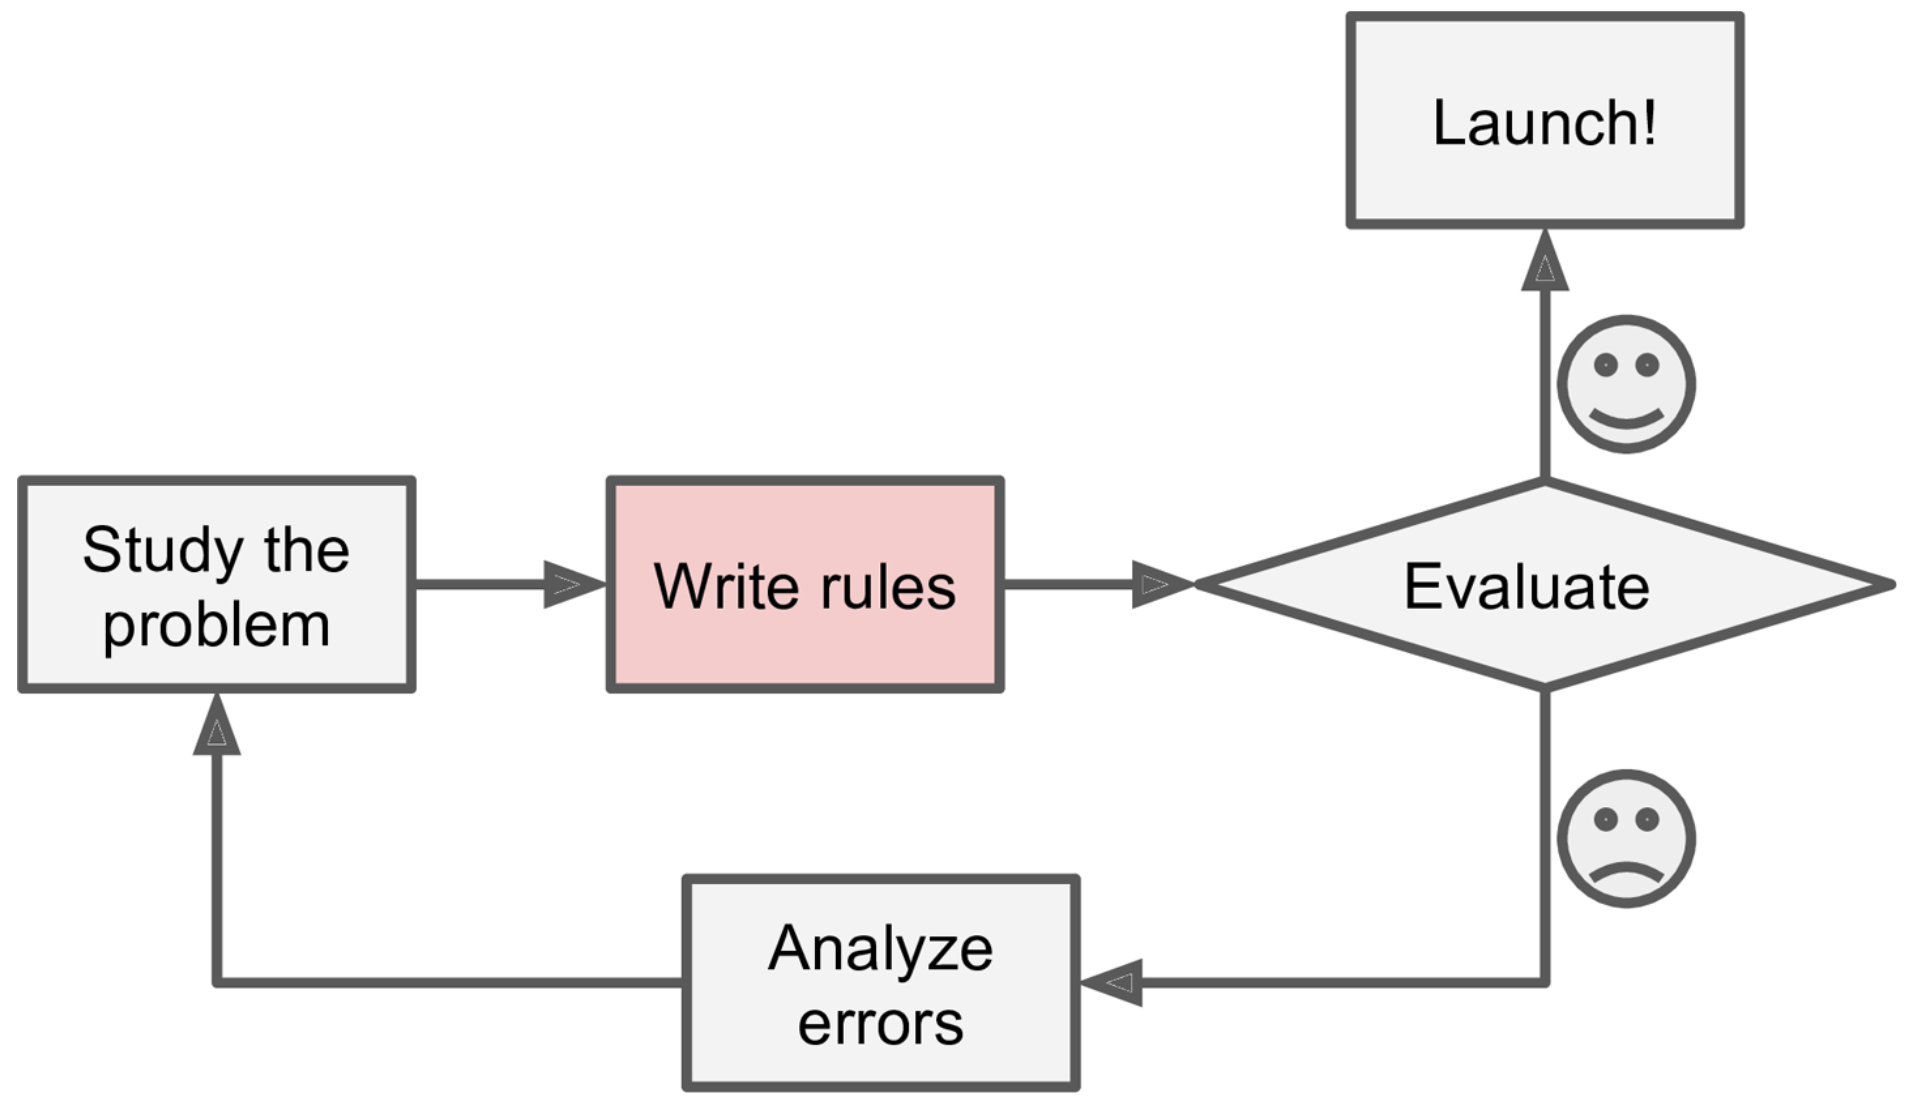
\includegraphics[height=0.7\textheight]{figures/geron-fig1-1}\let\thefootnote\relax\footnotetext{\tiny{Fig 1-1 from \emph{Hands-On Machine Learning with Scikit-Learn and TensorFlow} by Aurelien Geron (2017).}}
\par\end{center}

\end{frame}

\begin{frame}{Rule-Based Systems}

Issues with rule-based systems:
\begin{itemize}
\item Very labor intensive to build.
\item Rules work very well for areas they cover, but \textbf{cannot generalize} to unanticipated input combinations. 
\item Don't naturally handle uncertainty.
\item Expert systems seen as brittle
\end{itemize}
\end{frame}

\begin{frame}{Modern AI: Machine Learning}
\begin{itemize}
\item Don't reverse engineer an expert's decision process.

\item Machine \textbf{learns} on its own.

\item We provide \textbf{training data}:
many examples of (input $x$ , output $y$) pairs, e.g.

\begin{itemize}
\item A set of videos, and whether or not each has a cat.
\item A set of emails, and whether or not each is SPAM. 
\end{itemize}

\item Learning from training data of this form is called \textbf{supervised
learning}.
\end{itemize}
\end{frame}

\begin{frame}{Machine Learning Algorithm}
\begin{itemize}
\item A \textbf{machine learning algorithm} learns from the training data:
\begin{itemize}
\item \textbf{Input}: Training Data
\item \textbf{Output}: A prediction function that produces output
$y$ given input $x$.
\end{itemize}

\item The success of ML depends on
    \begin{itemize}
        \item Availability of large amounts of data
        \item \textbf{Generalization} to unseen samples (the test set)
    \end{itemize}
\end{itemize}
\end{frame}

\begin{frame}{Machine Learning Approach}
\begin{center}
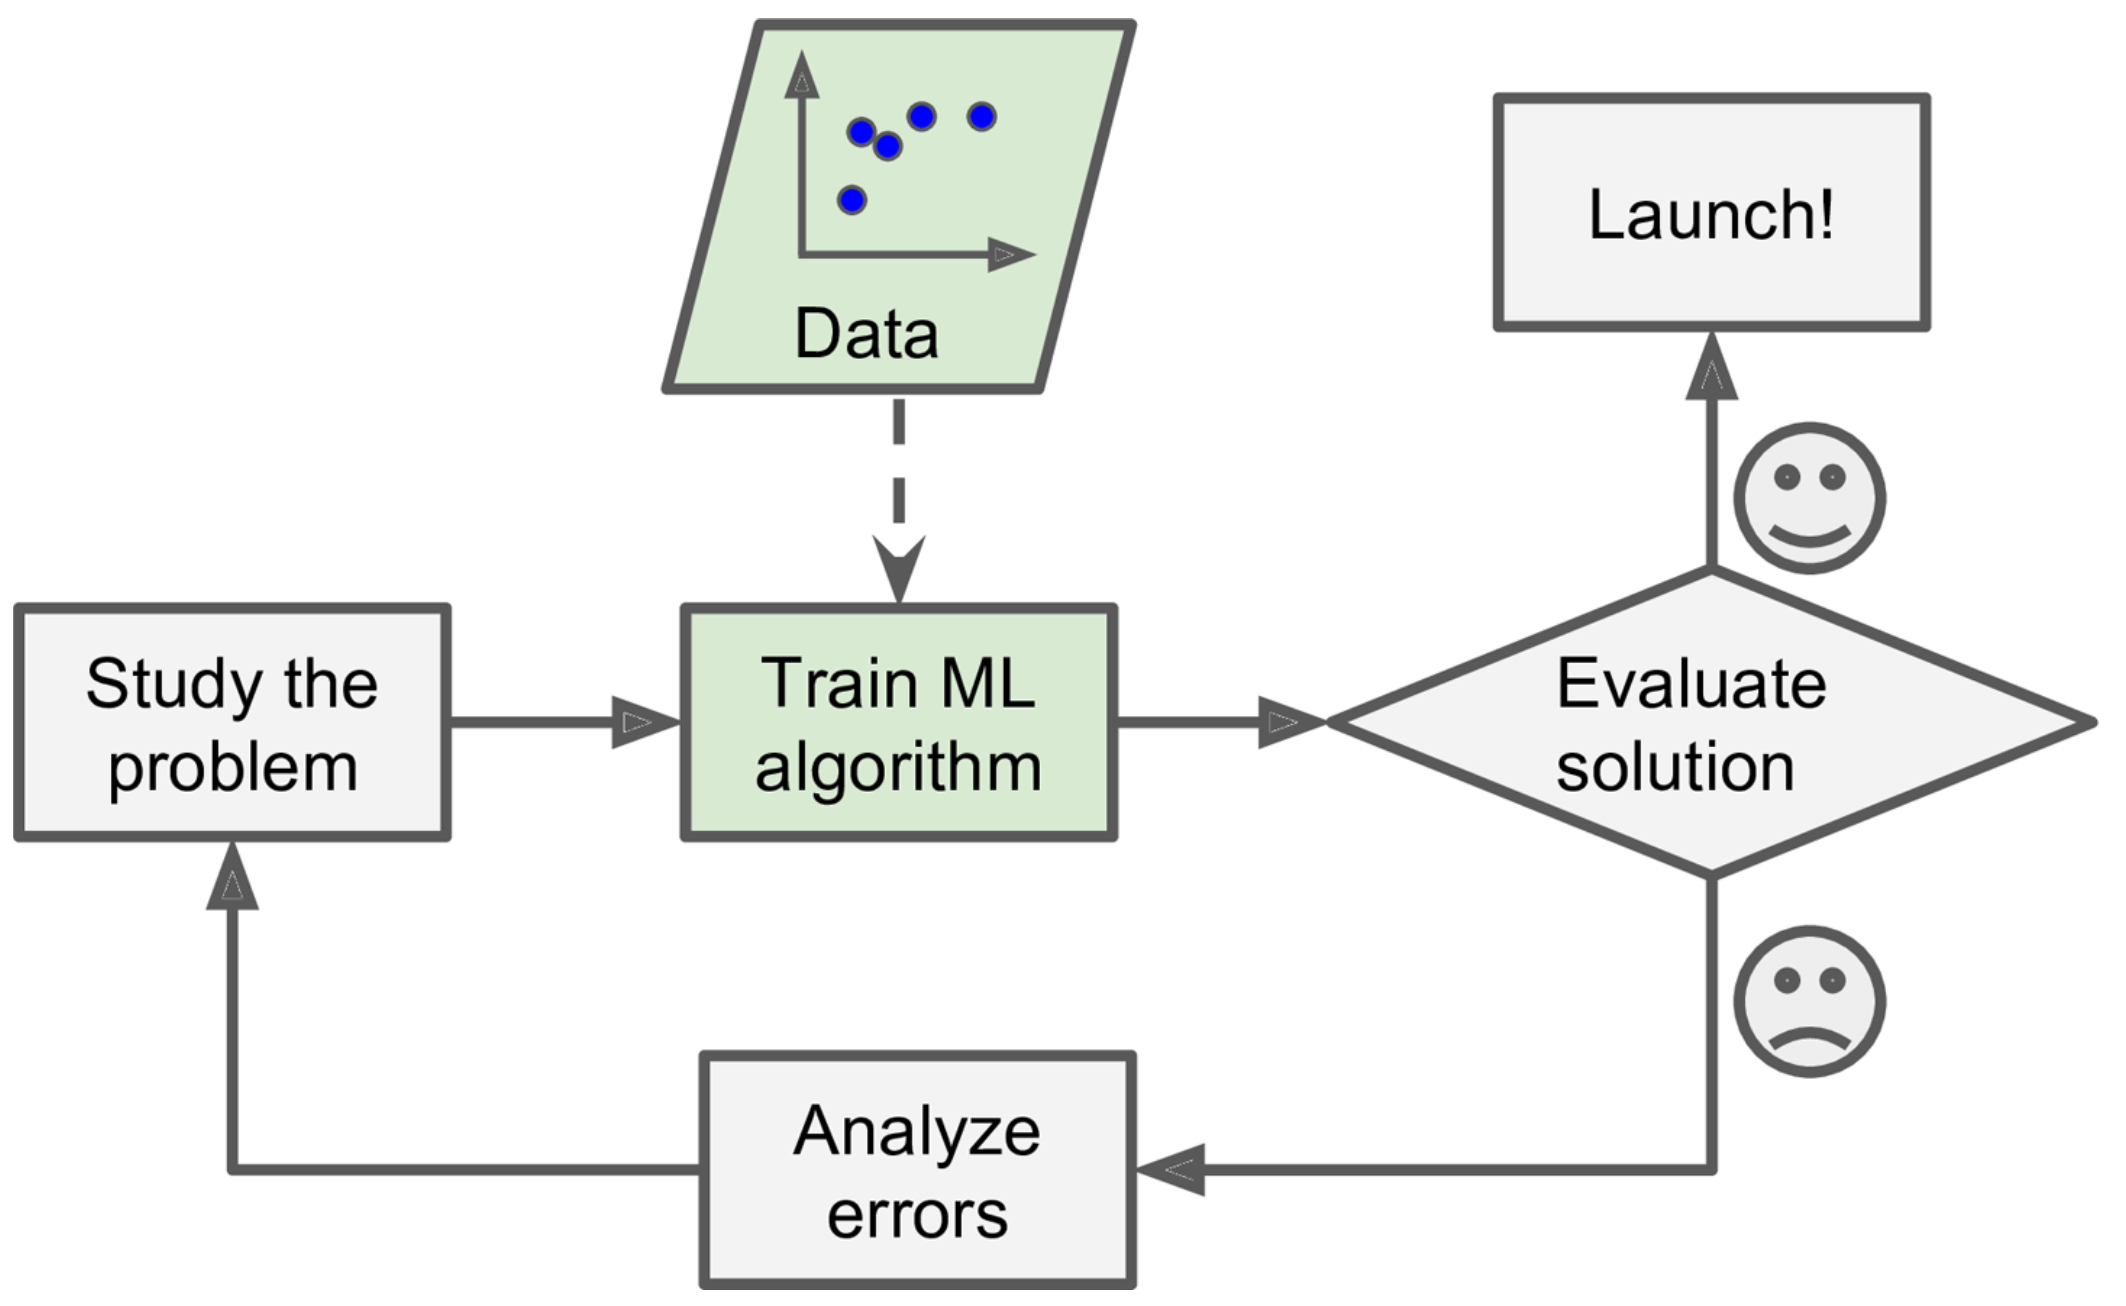
\includegraphics[height=0.7\textheight]{figures/geron-fig1-2}
\par\end{center}

\mode<article>{We've swapped out rule writing with ``machine learning.'' But how
does adjust the ML training process by analyzing errors?}
\begin{center}
\let\thefootnote\relax\footnotetext{\tiny{Fig 1-2 from \emph{Hands-On Machine Learning with Scikit-Learn and TensorFlow} by Aurelien Geron (2017).}}
\par\end{center}

\end{frame}

\begin{frame}{Key concepts}
\begin{itemize}
    \item Most common \textbf{ML problem types}

\begin{itemize}
    \item classification (binary and multiclass)
\item regression
\end{itemize}

\item \textbf{prediction function}: predicts output $y$ given input $x$
\item \textbf{training data}: a set of (input $x$, output $y$) pairs
\item \textbf{supervised learning algorithm}: takes training data and produces a prediction function
\item Beyond prediction
    \begin{itemize}
        \item \textbf{Unsupervised learning}: finding structures in data, e.g. clustering
        \item \textbf{Reinforcement learning}: optimizing long-term objective, e.g. Go  
        \item \textbf{Representation learning}: learning good featurs of real-world objects, e.g. text
    \end{itemize}
\end{itemize}
\end{frame}

\begin{frame}
    {Core Questions in Machine Learning}
    Given any task, the following questions need to be answered:
    \begin{itemize}
        \item \textbf{Modeling}: What is the prediction function?
        \item \textbf{Learning}: How to learn the prediction function from data?
        \item \textbf{Inference}: Given a learned model, how to make predictions?
    \end{itemize}
\end{frame}

\end{document}
